\hspace{1.5cm}
\FloatBarrier
\begin{figure}[!htpb]
        \centering
        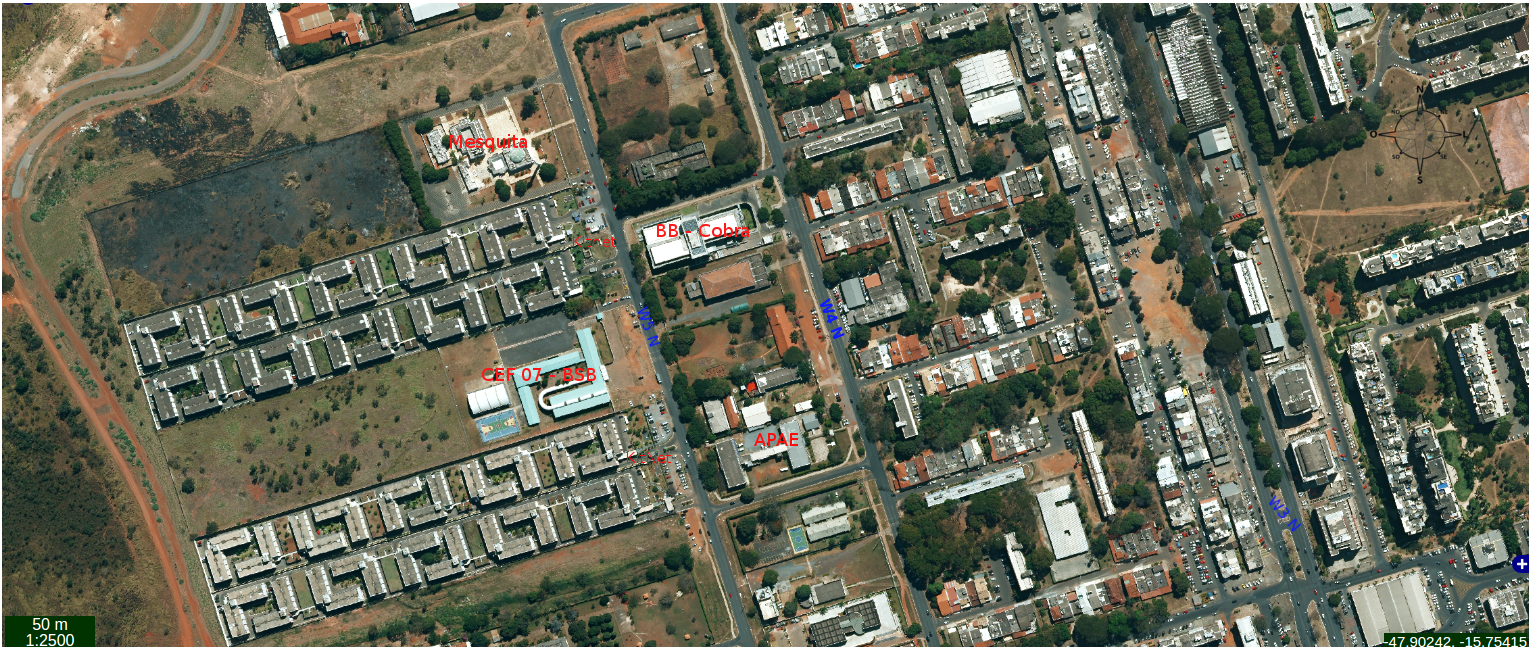
\includegraphics[width=1\textwidth]{imagens/CEF07Bsb.png}
        \caption{Vista aérea da região do Centro de Ensino Fundamental nº 07 de Brasília.}
        \label{figura01}
\end{figure}
\FloatBarrier

\paragraph{}O Centro de Ensino Fundamental nº 07 de Brasília, está localizado na quadra 912 Norte, entre o bairro do Noroeste e a 712 norte, no bairro da Asa Norte/Brasília/DF. Esta nova construção substituiu a antiga escola, que localizada na 711 norte. No seu lado esquerdo e direito temos dois conjuntos de KitNet, bem como um conjunto de escolas particulares e a Mesquita Islâmica. O Parque do recém criado bairro Noroeste, faz divisa com sua parte posterior. Na imagem de satélite, figura \ref{figura01}, este fato é melhor exemplificado. A escola tem seu perímetro cercado, bem como uma separação entre as áreas construida e verde. Sua segurança é constituída por 01 (um) vigilante e câmaras de segurança espalhadas pelo corredores, bem como ronda do Batalhão escolar.
\begin{figure}[!htpb]
        \centering
        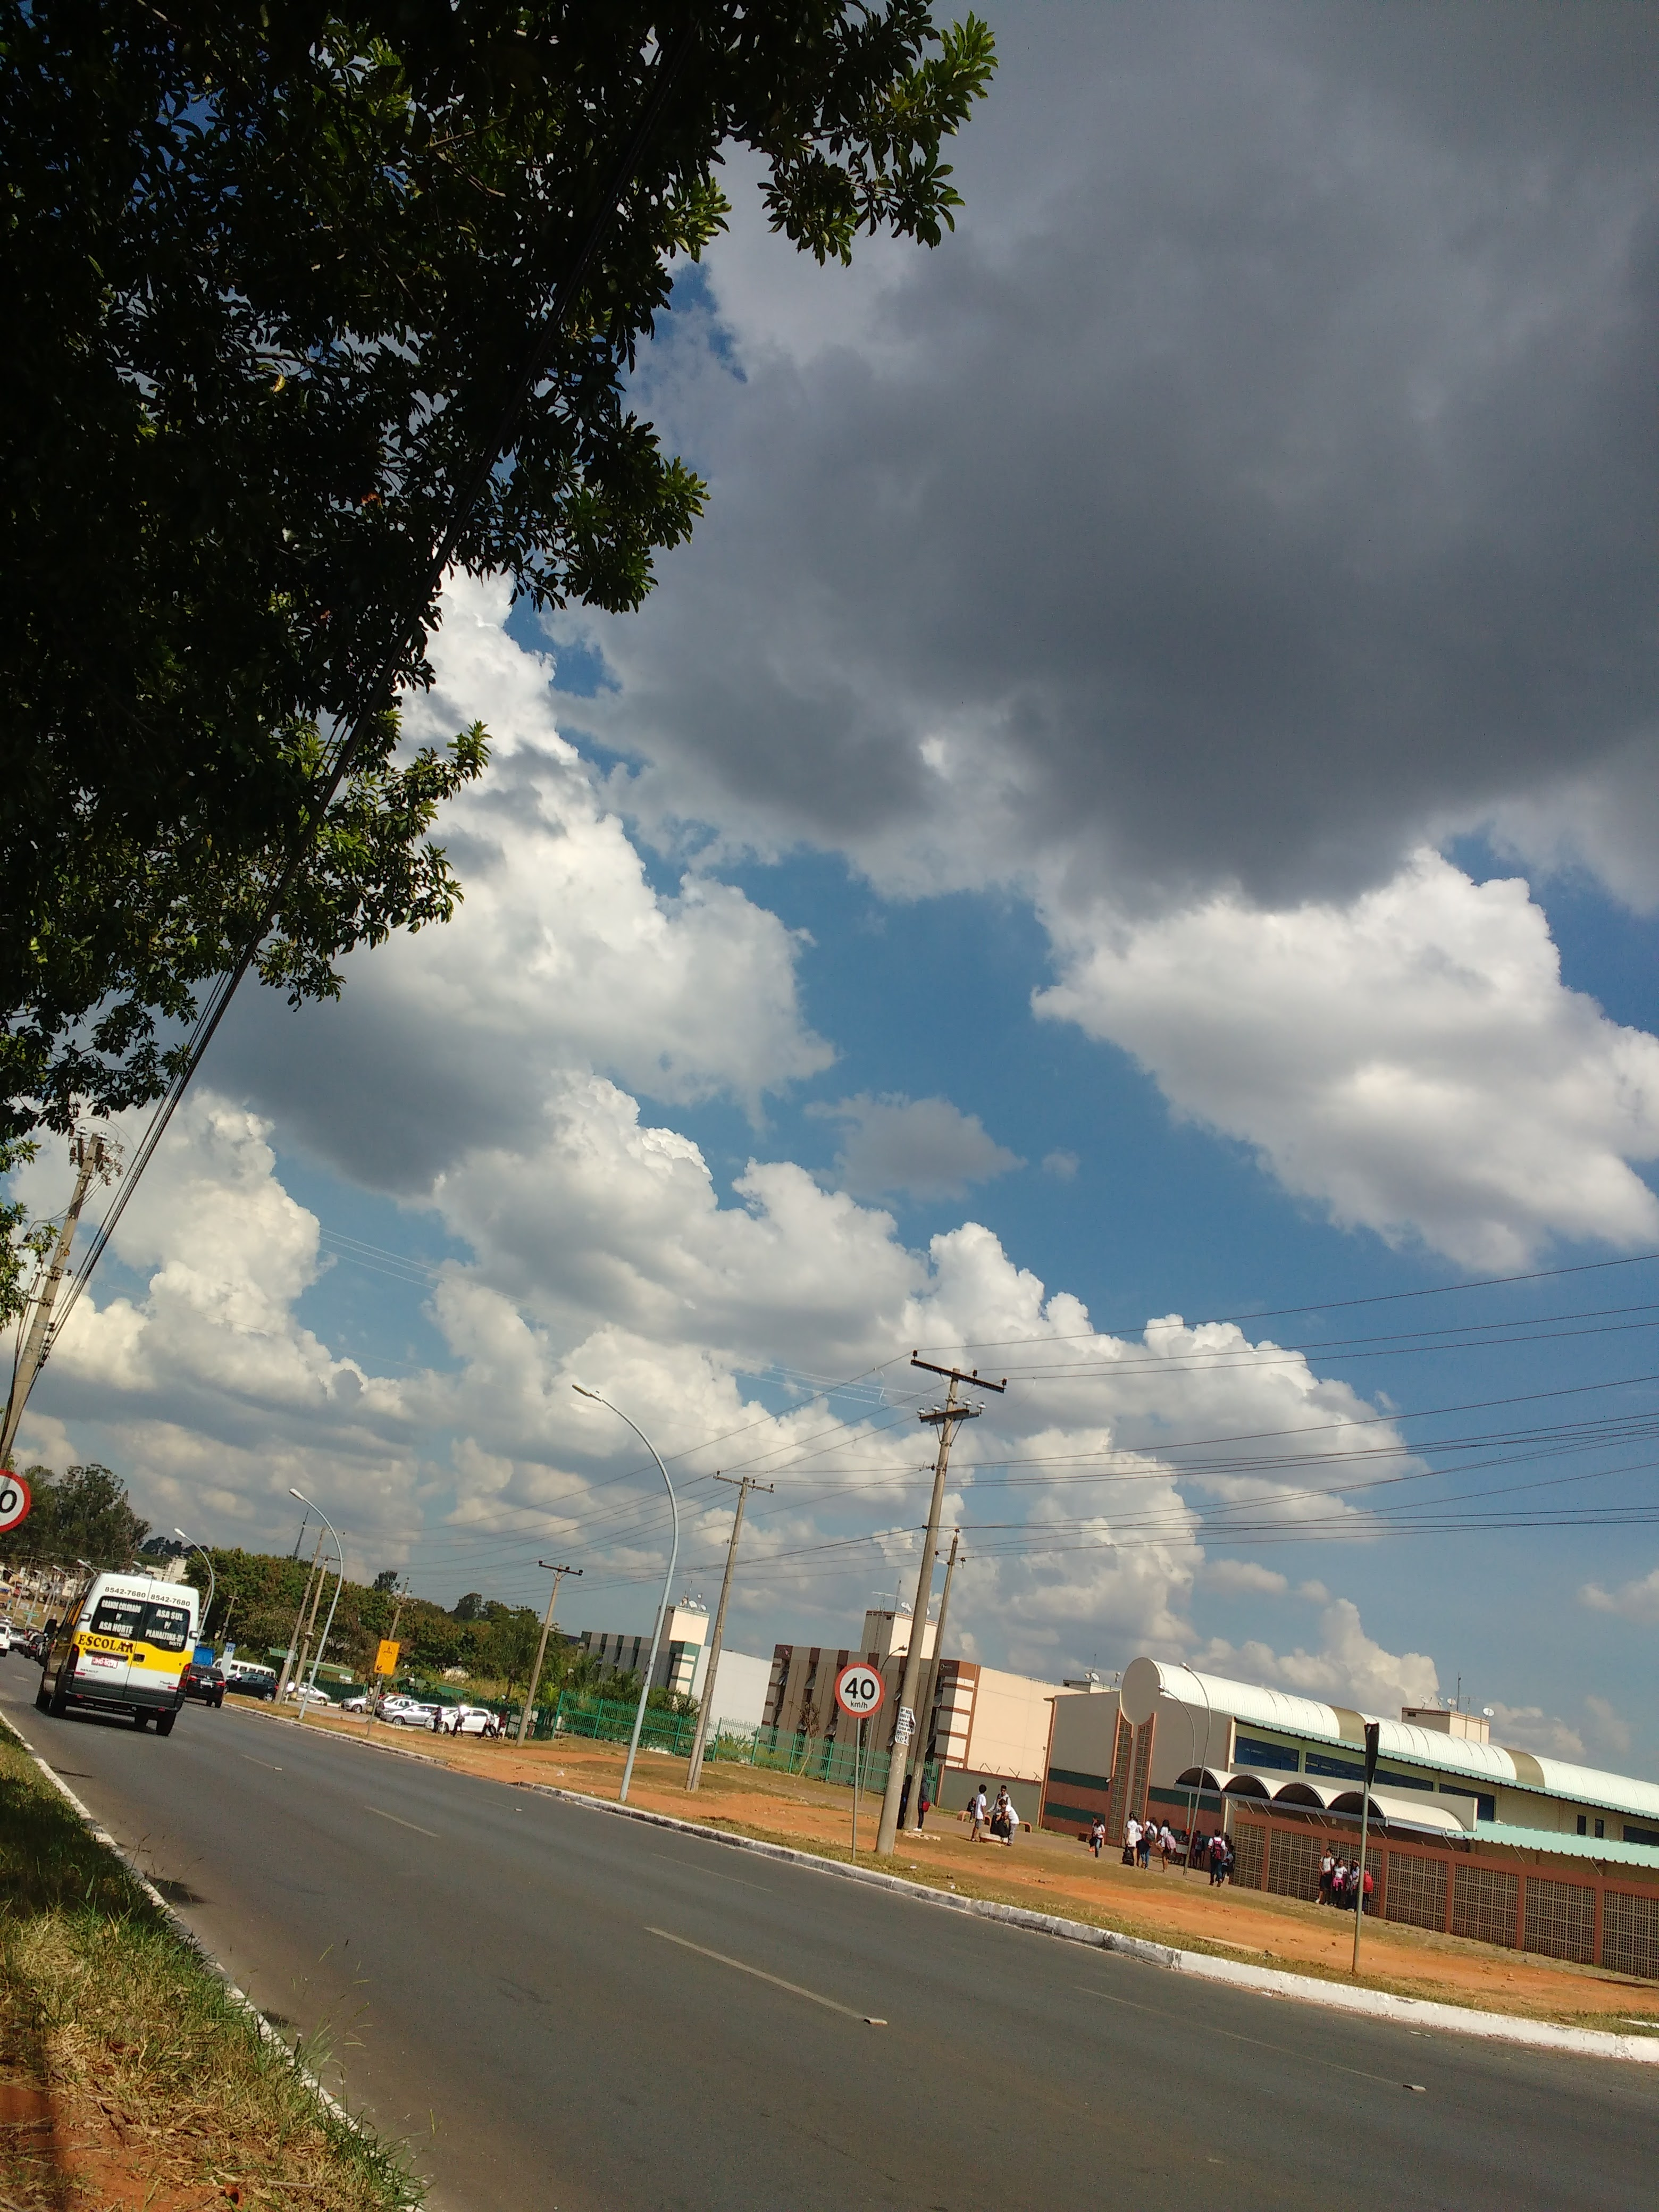
\includegraphics[width=.7\textwidth, height=.3\textheight]{imagens/13-01-07_10-06-2016.jpg}
        \caption{Centro de Ensino Fundamental nº 07 de Brasília.}
        \label{figura02}
\end{figure}
\paragraph{}Já sua fachada está localizada na rodovia  W5  norte, atrás do escritório do banco do Brasil,  APAE  e  algumas  igrejas.  Está  rodovia  tem  um  fluxo  constante  de  veículos,  com aumento  de  intensidade  na  parte  da  manhã  e  noite.  Este  fato  se  dar  devido  a  saída  dos moradores,  dos  dois  conjunto  de  kitNet.  Outro  fato  que  eleva  a   ocorrência  de  veículos, principalmente  no  período  noturno,  é  chegada  dos  moradores,  os  frequentadores  da Mesquita  e  das  Igrejas  (evangélicas   e  Espirita),  existente  no  local.  A  escola  não  possui atividade  durante  o   período  noturno.  Seus  turno  estão  dividido  da  seguinte  forma:  8º  e  9º ano no período matutino; e os alunos da 6º e 7º ano no período vespertino. Na sua entrada os alunos fazem sua concentração na frente da escola só podendo adentrar as instalações o toque do sinal, figura \ref{figura02}. Cada turno tem 6 (seis) horário, com um intervalo entre o terceiro e quarto. Durante este intervalo os realizam  diversas brincadeira, vão a lanchonete \footnote{A lanchonete é o local disputado pelo estudante, pois nela a variedade de lanche é maior do que na cantina. Cada estudante gasta em média de R\$ 2,50 à 5,00 na compra de salgados e doces.} (figura \ref{figura07}) e a cantina, enquanto os professores utiliza este momento para realizar sua confraternizações diversas, na sala dos professores.  
\FloatBarrier
\begin{figure}[!htpb]
        \centering
        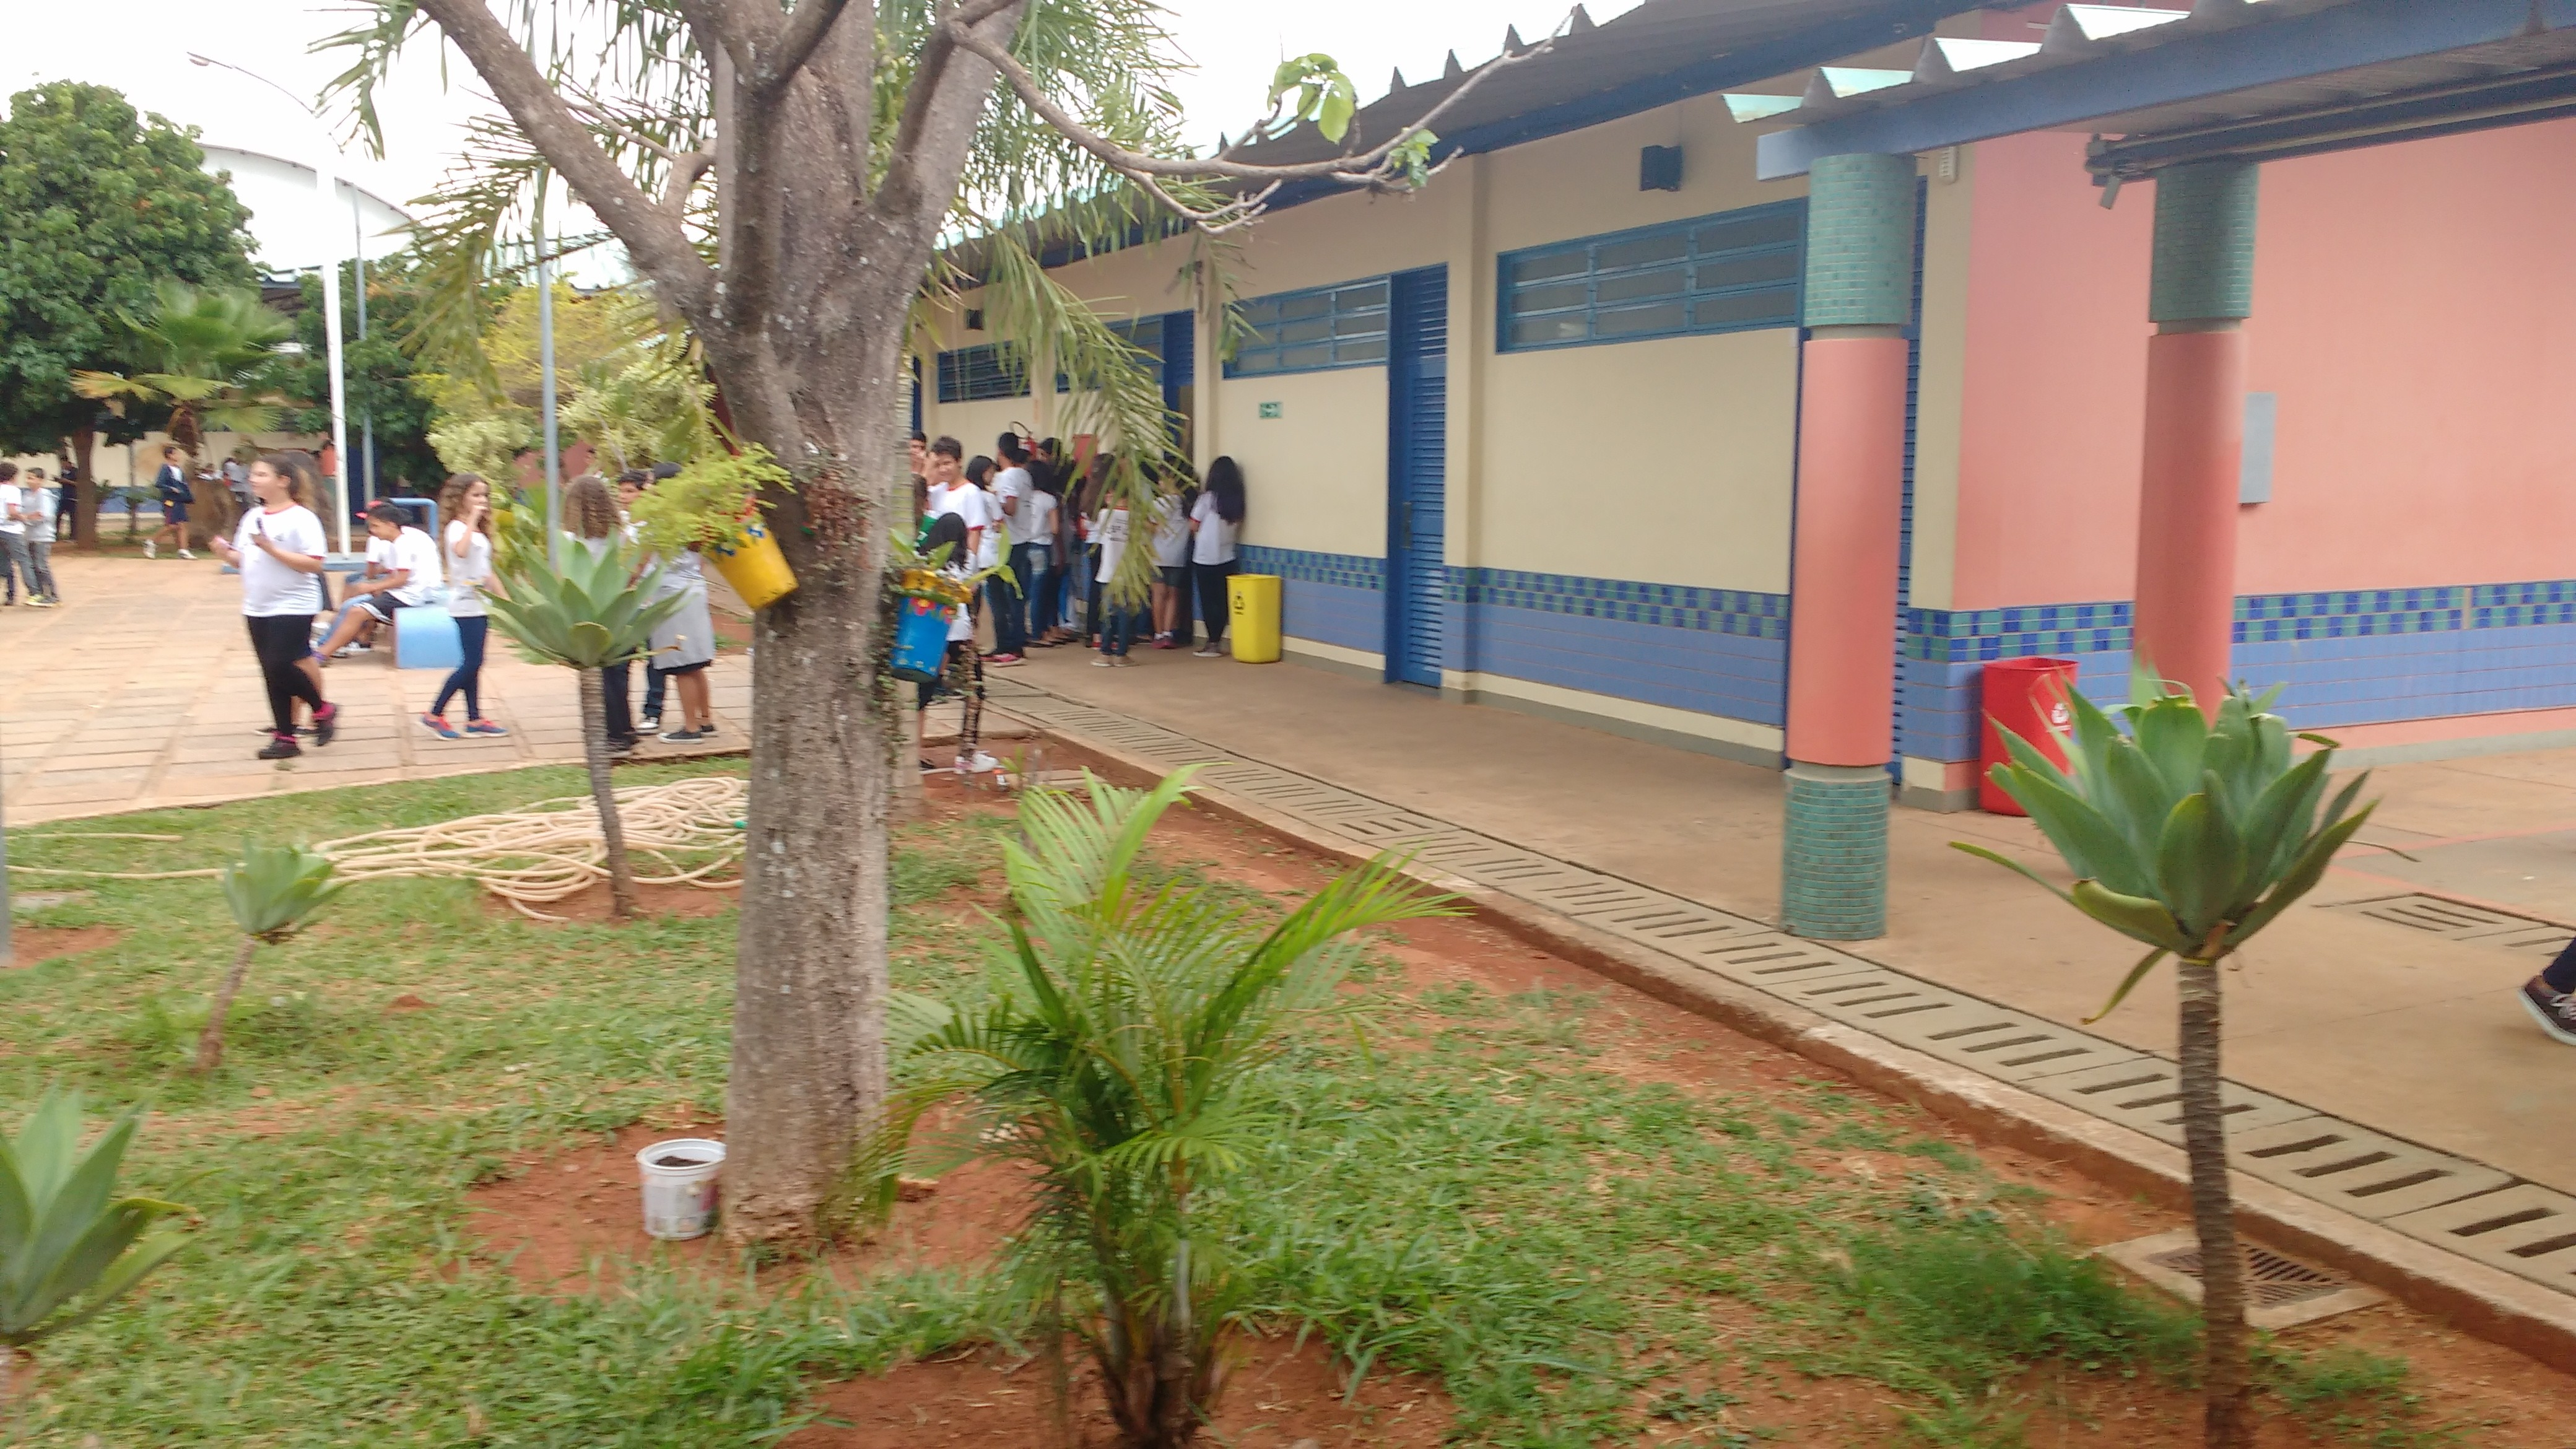
\includegraphics[width=.7\textwidth]{imagens/IMG_20161018_154304252.jpg}
        \caption{Fila na lanchonete, para compra de salgados.}
        \label{figura07}
\end{figure}
\FloatBarrier

\begin{figure}[!htpb]
\begin{center}
	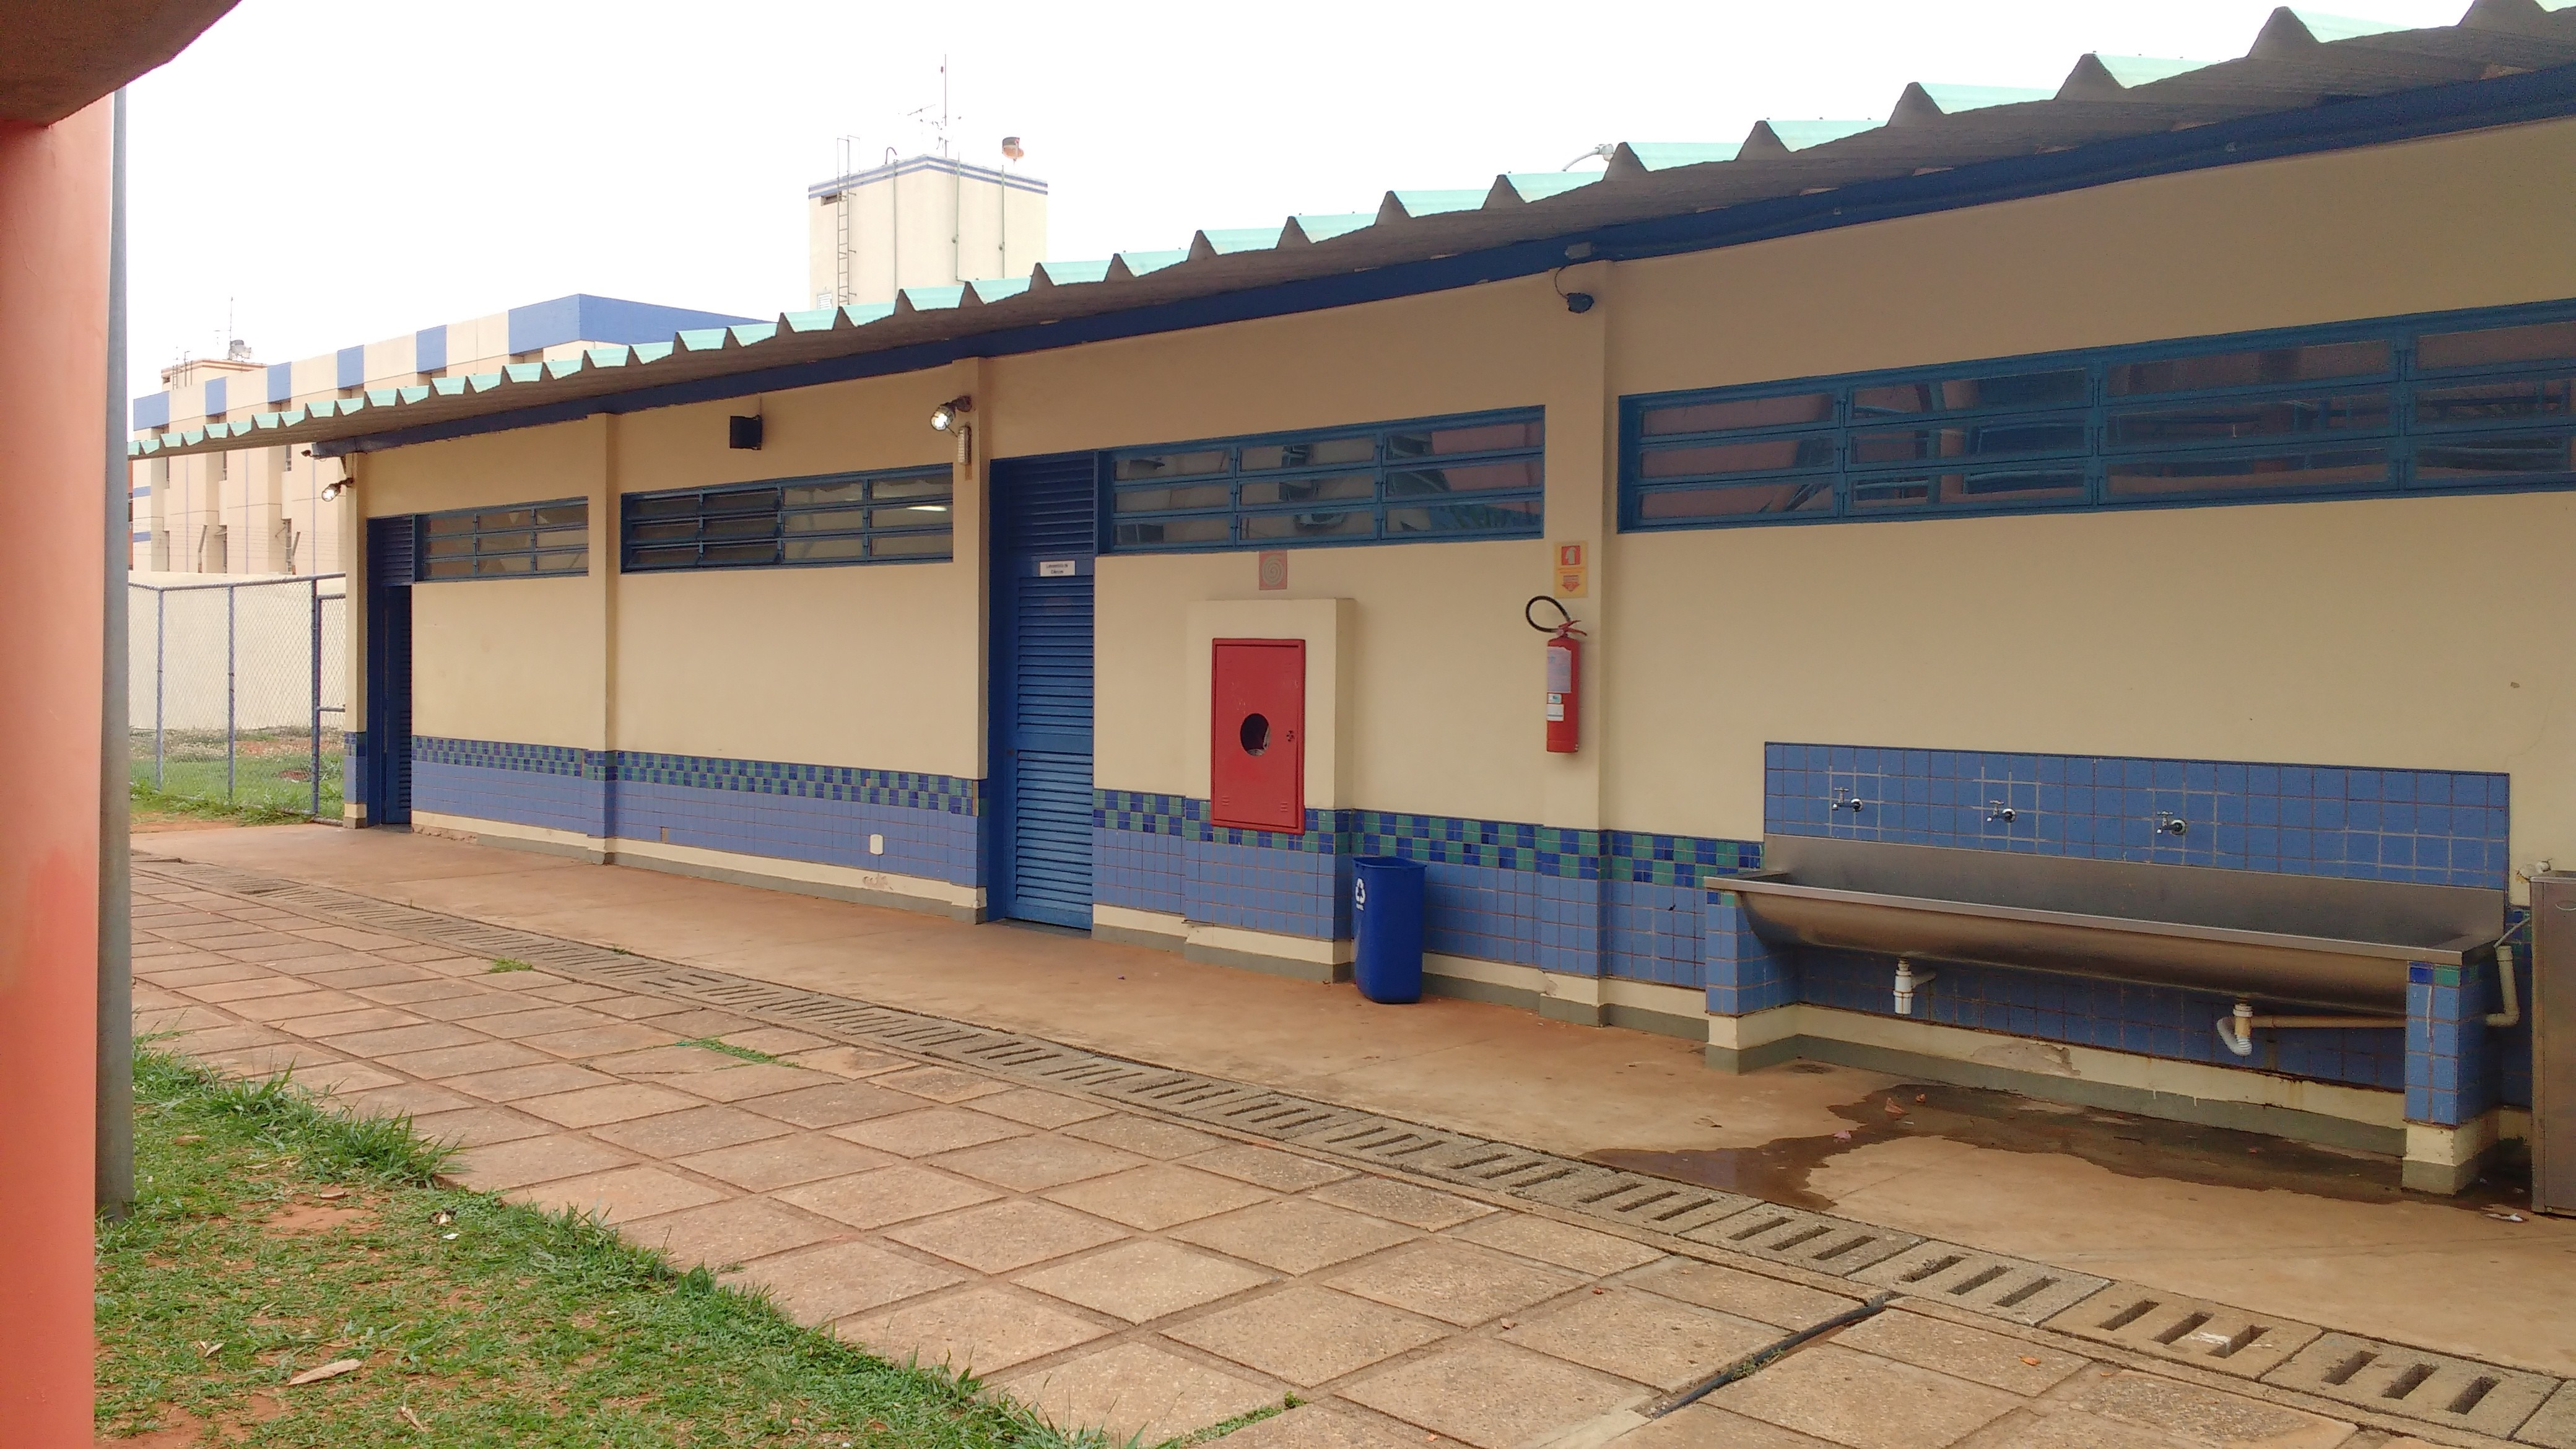
\includegraphics[width=.6\textwidth]{imagens/IMG_20161018_162635672.jpg} \quad
	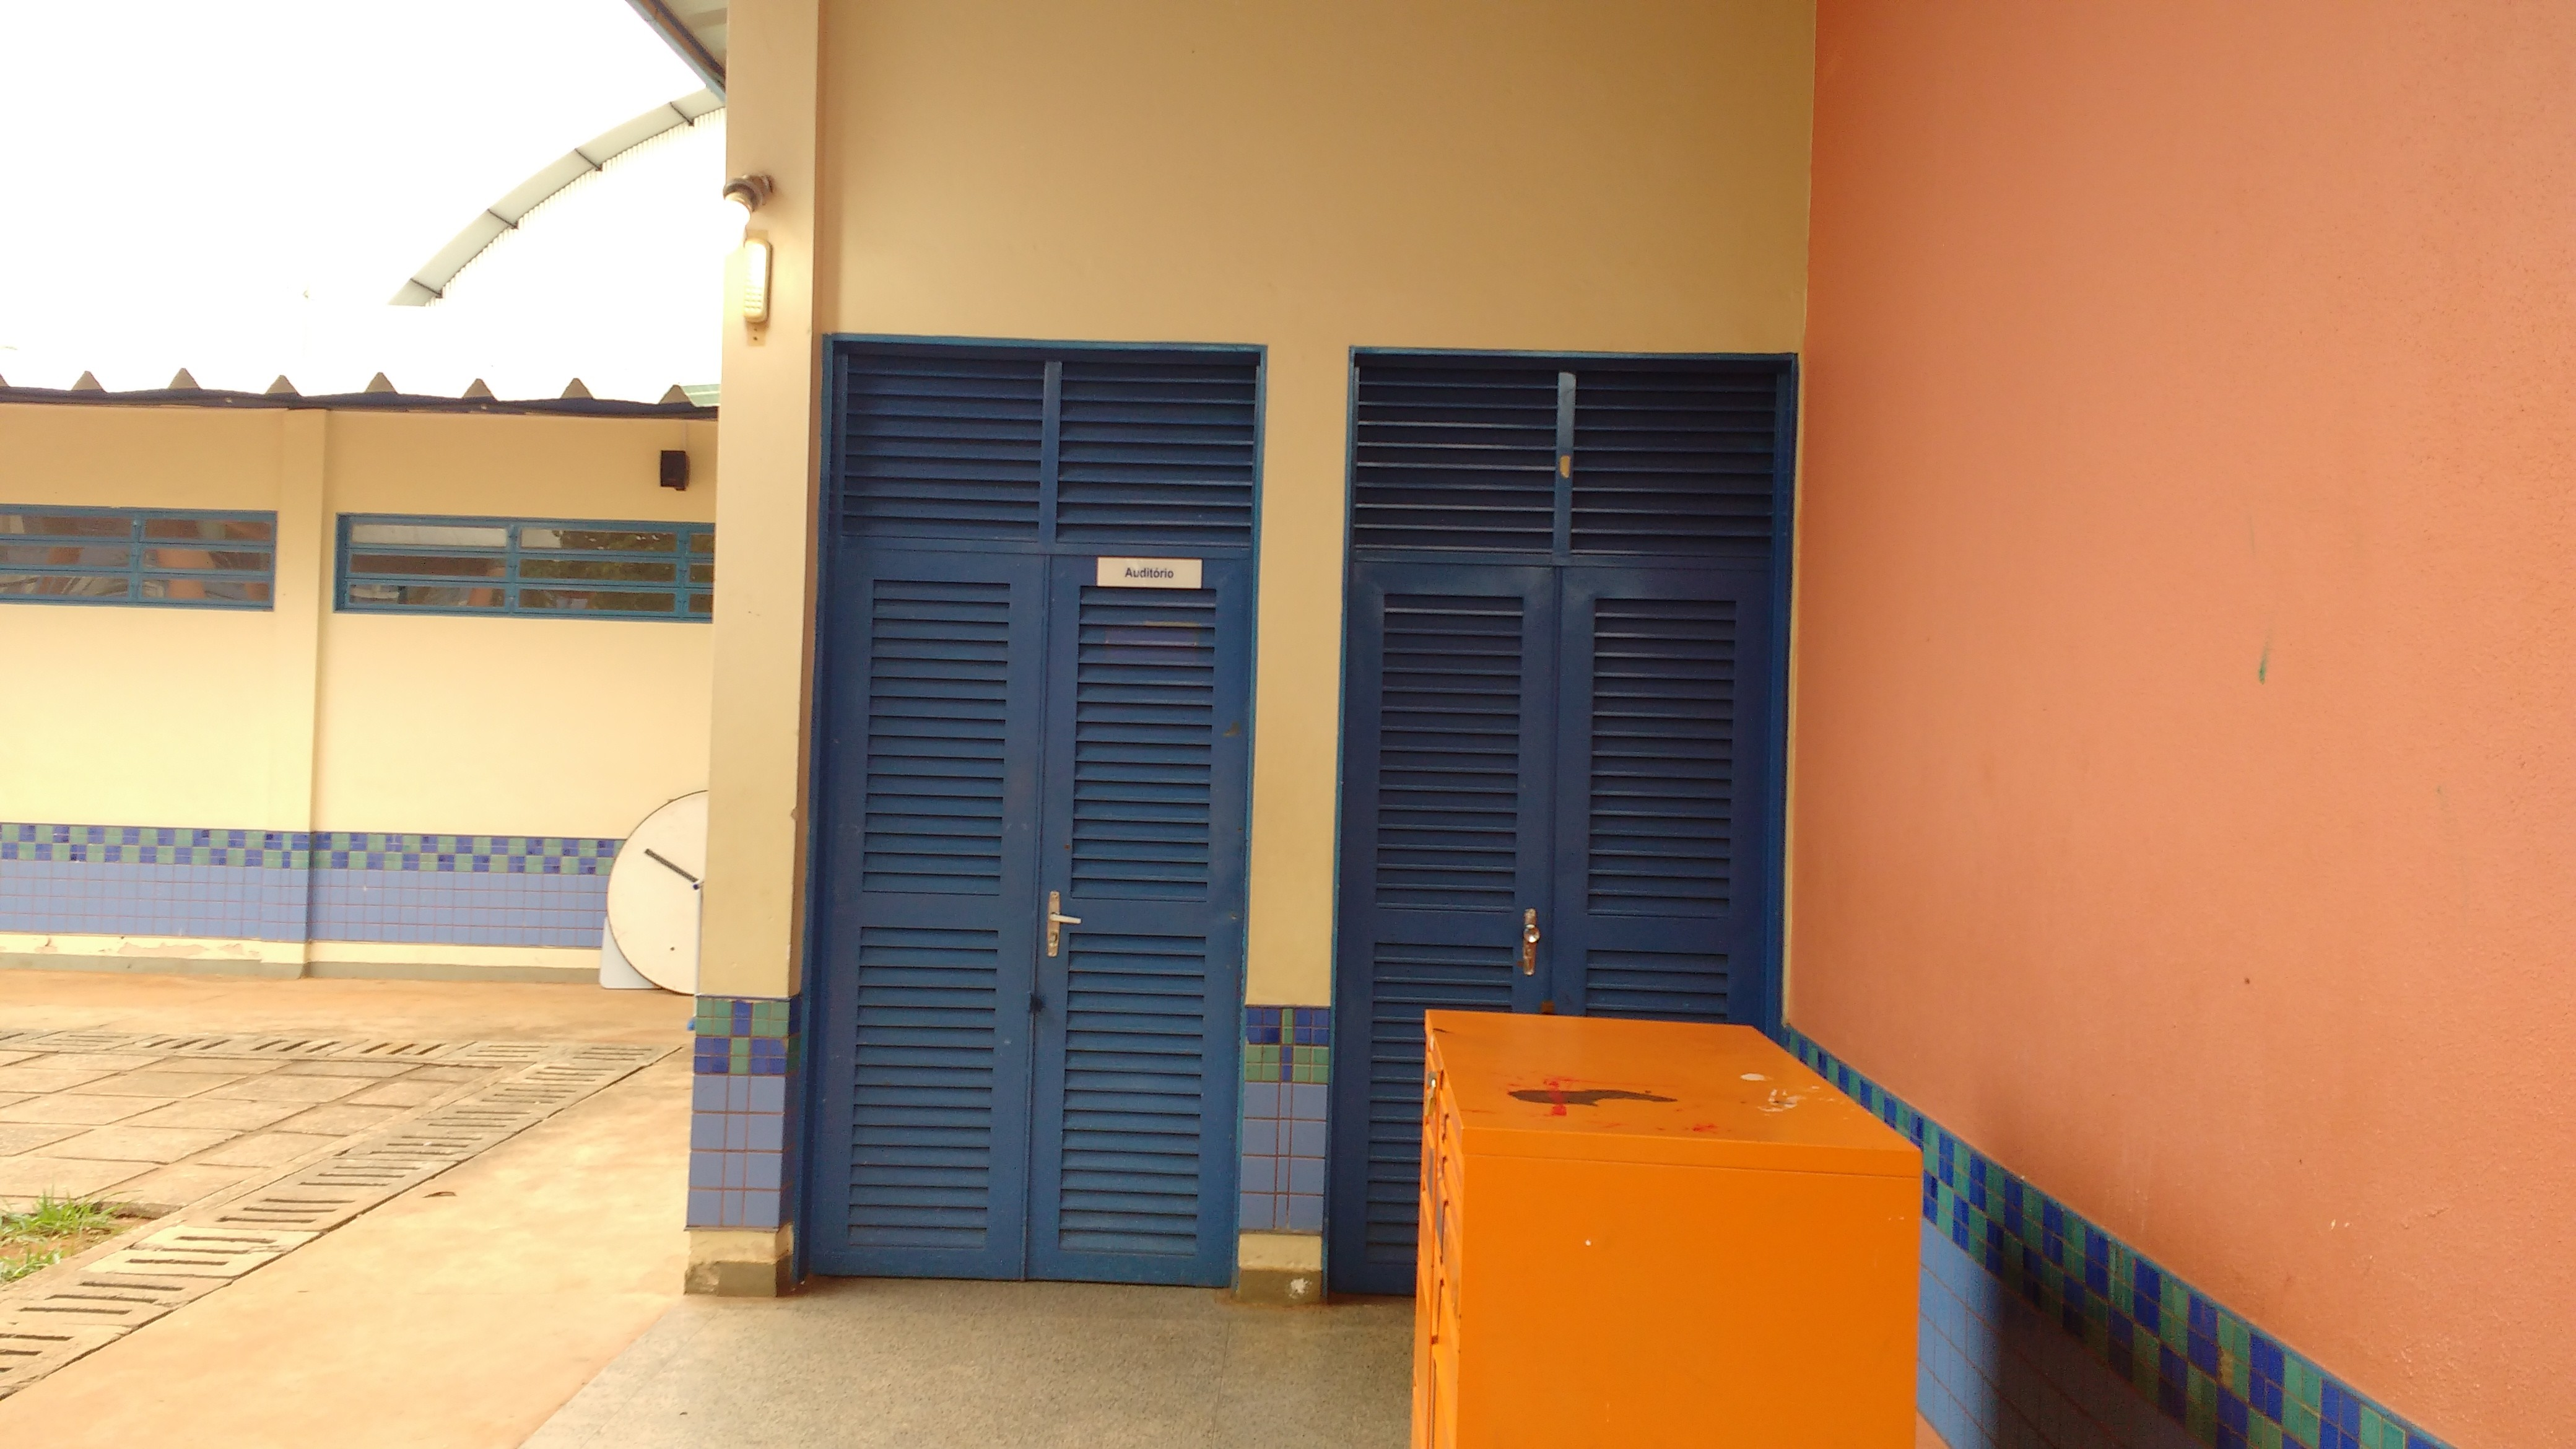
\includegraphics[width=.6\textwidth]{imagens/IMG_20161018_162545314.jpg}
\caption{Área de laboratórios, recursos e Auditório} \label{figura08}
\end{center}
\end{figure}

\begin{figure}[!htpb]
        \centering
        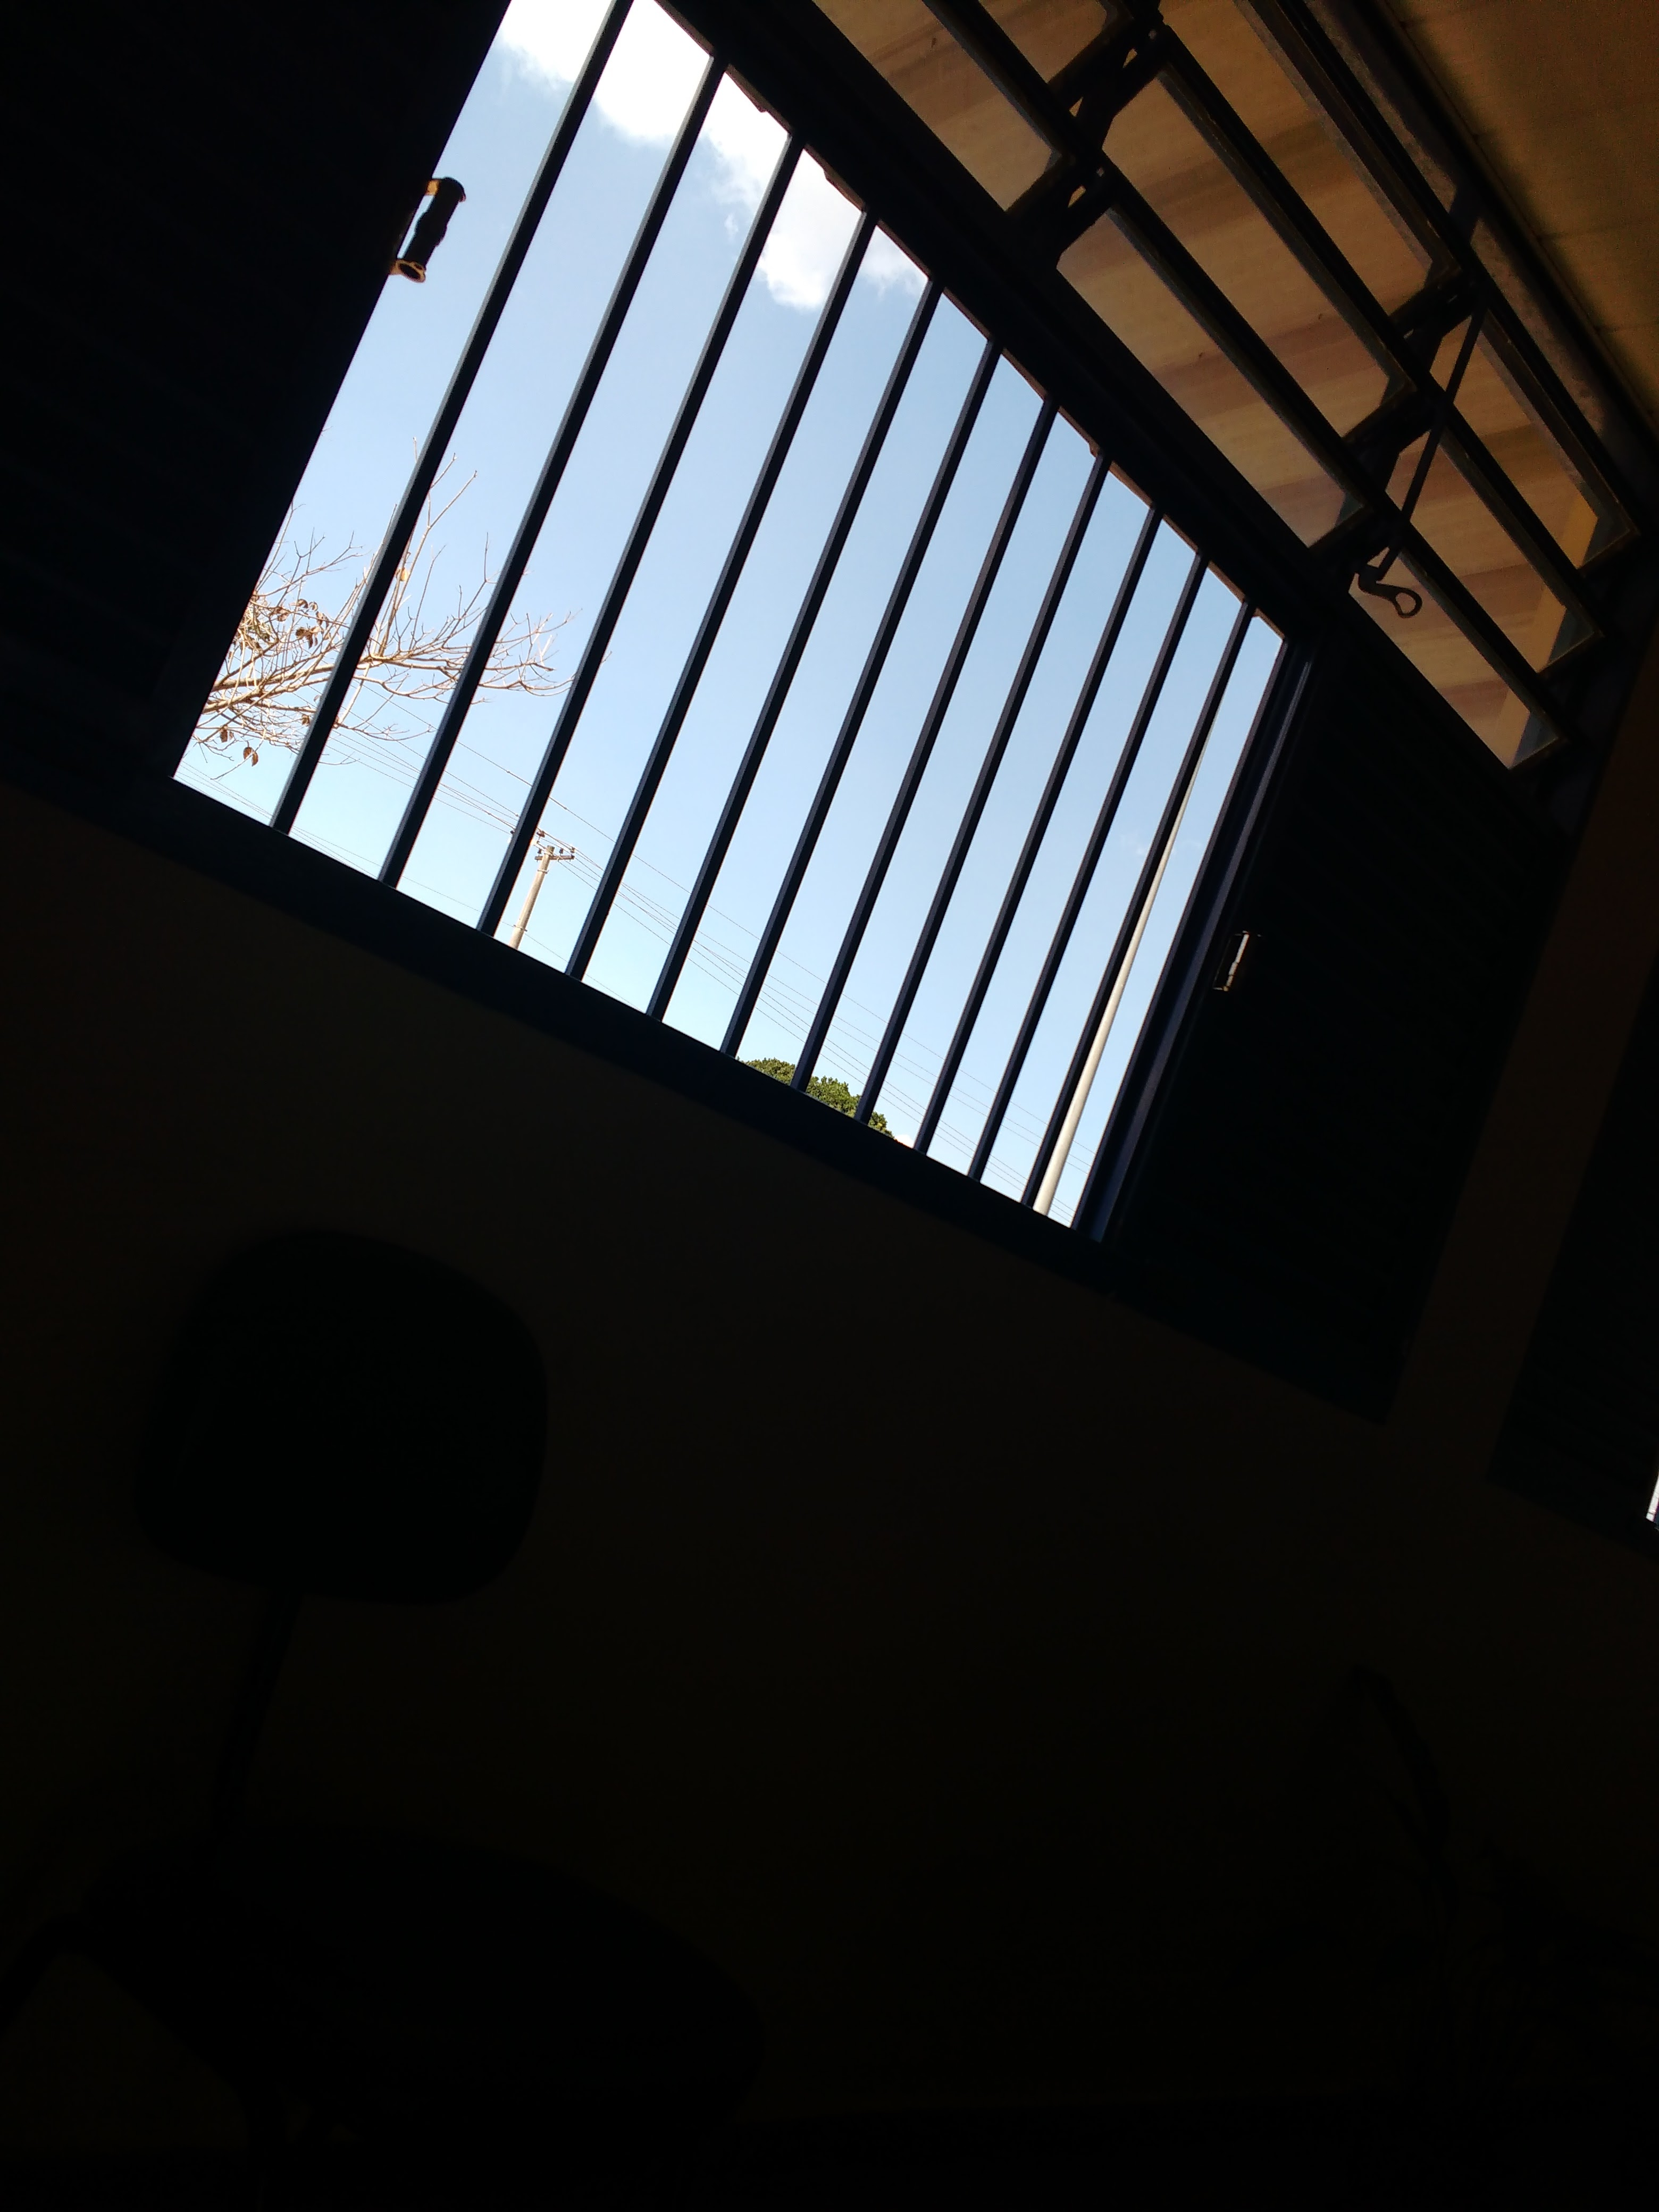
\includegraphics[width=.5\textwidth]{imagens/13-08-04_10-06-2016.jpg}
        \caption{Janelas gradeadas, sala de aula.}
        \label{figura03}
\end{figure}

\paragraph{}Sua  infraestrutura  é  bem  organizada  com Laboratório,   auditório,  biblioteca, sala de leitura,  ginásio  de  esporte, sala de recursos, SOE, conforme figura \ref{figura08}.  Nas  sala  de  aulas  existente  meio  audiovisuais (televisão), quadros  (giz  e  caneta),  localizado  na  frente  e  fundo. As salas tem suas janelas gradeadas, dando uma ideia de encarceramento dos indivíduos (alunos e professores) durante as aulas, figura \ref{figura03}. Após  as  construções,  existe uma área verde  que  pode  ser explorado numa análise ambiental. Nesta área será criada uma pista de orientação  para  a  comunidade  escolar,  em  uma parceria  entre  a  Marinha  do  Brasil  e   a escola  (figura \ref{figura04}).  Apesar  do  comércio  e  algumas  residências  estarem  localizadas  a  uma quadra  de  distância  do  Centro  de  ensino,  nas  quadras  700,  suas  dinâmica  influência  no ambiente  escolar.  Isto  se  dar  no  ir  e  vim  dos  moradores  e  funcionários,  sendo  nas caminhadas/corridas,  nas  saídas  ou  chegada  de  sua residência/comércio  onde o deslocamento o leve pela W5, figura \ref{figura05}, que tem sentido único.
\begin{figure}[!htpb]
        \centering
        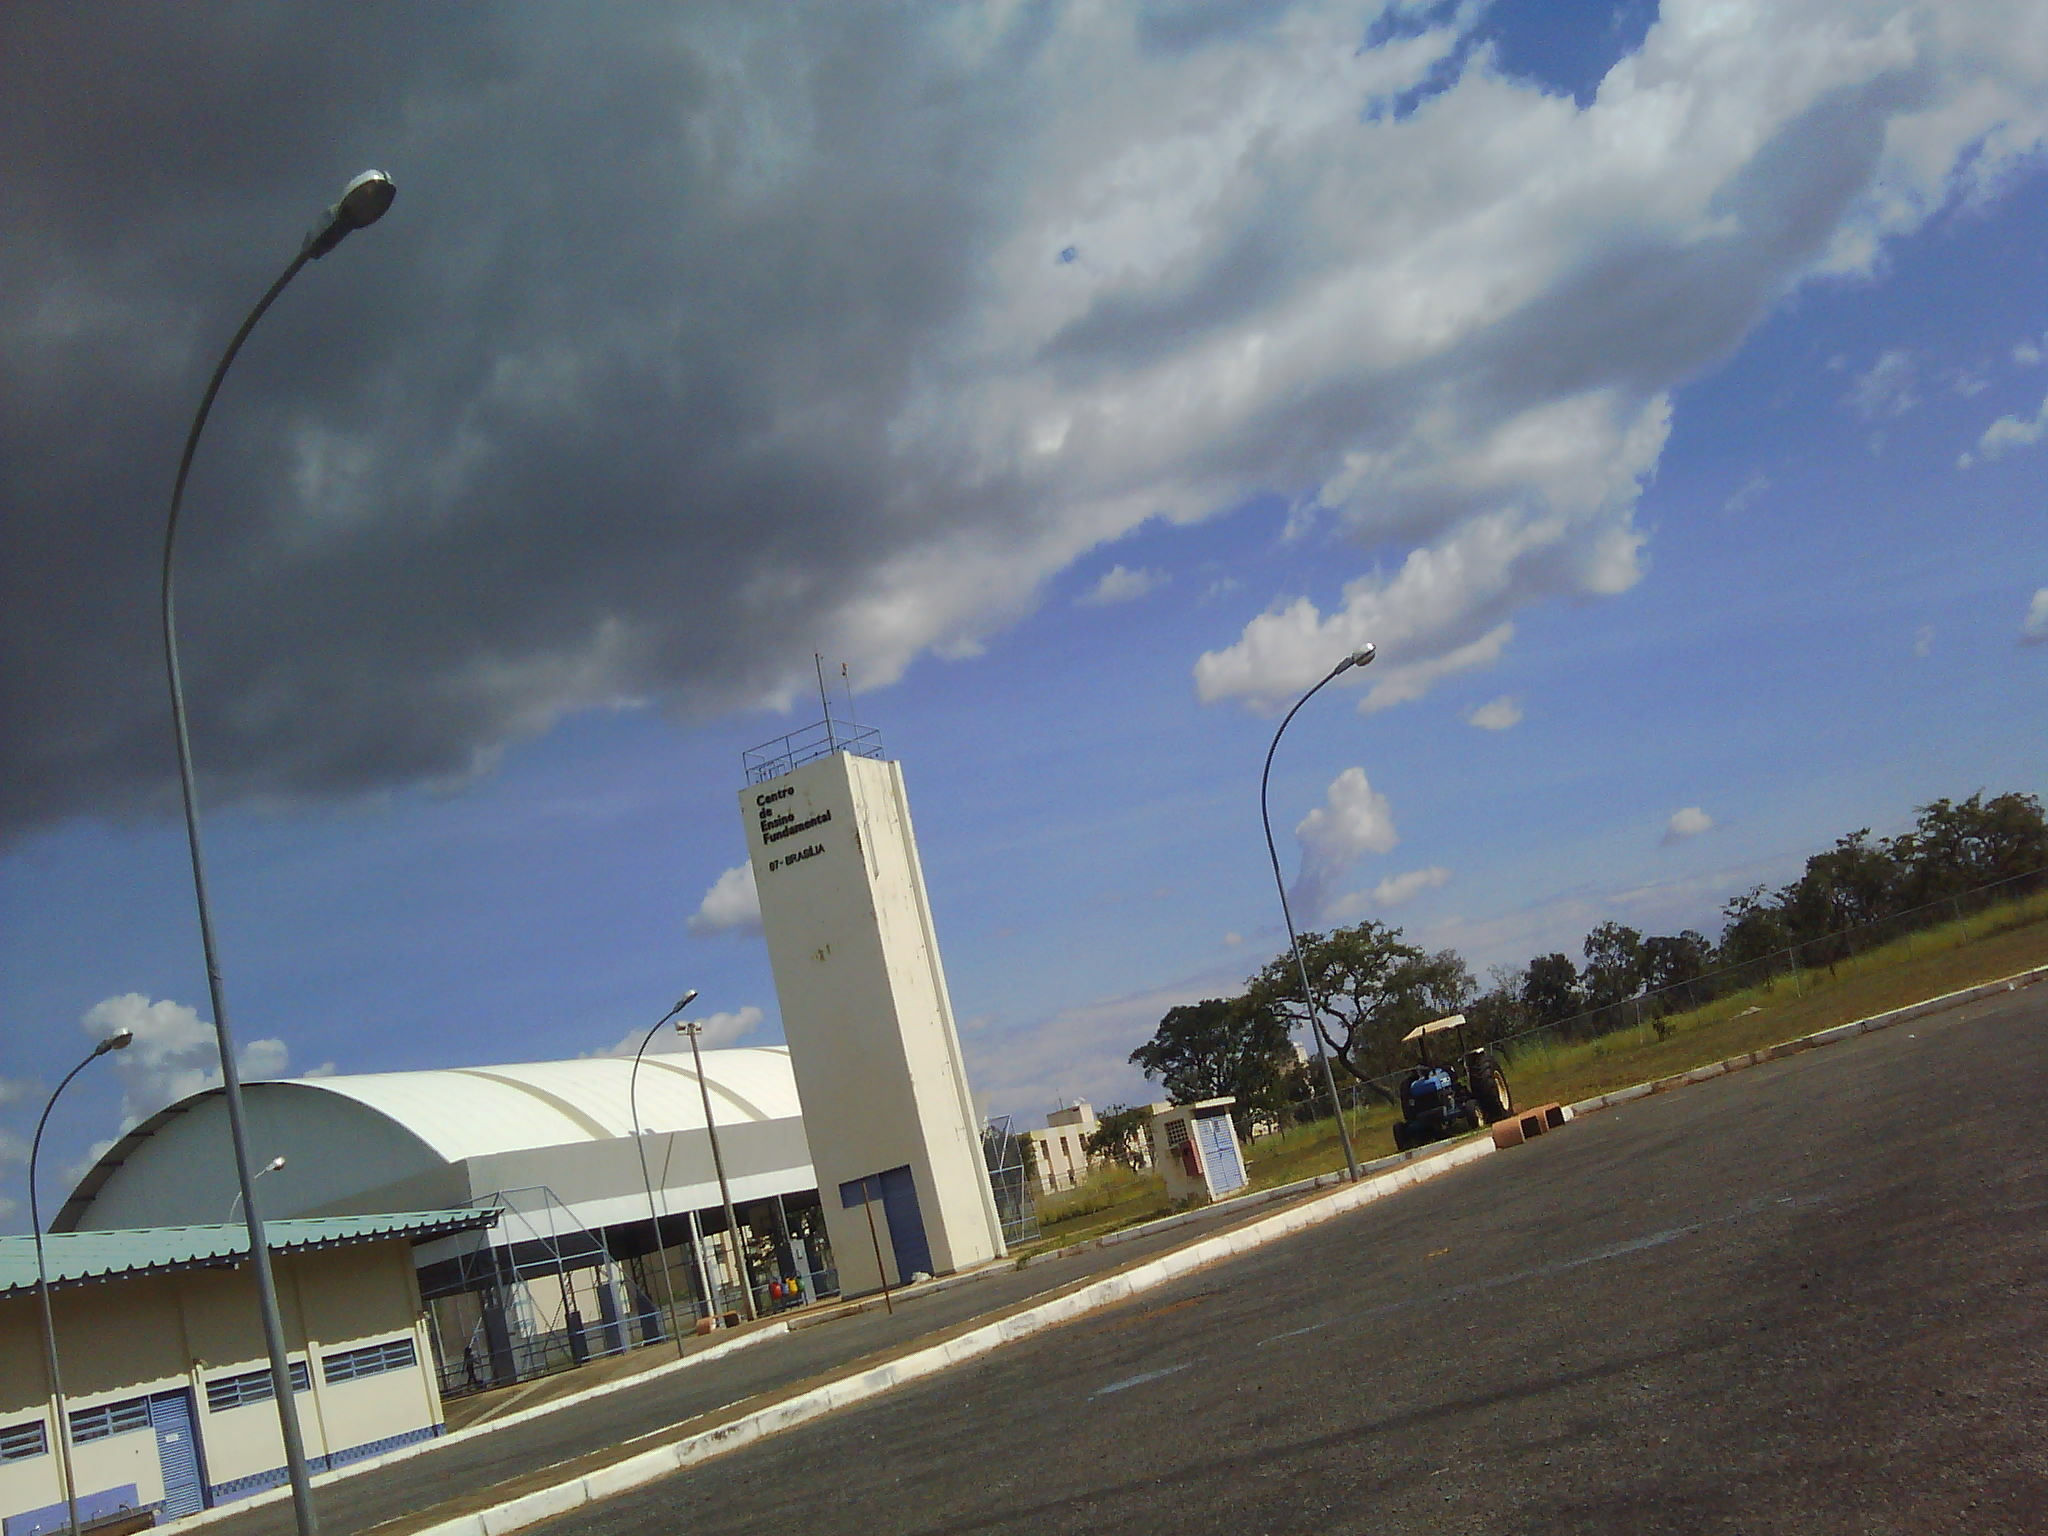
\includegraphics[width=.5\textwidth]{imagens/2016-06-03T16-12-23.jpeg}
        \caption{Área verde localizada na parte posterior na escola}
        \label{figura04}
\end{figure}
\begin{figure}[!htpb]
        \centering
        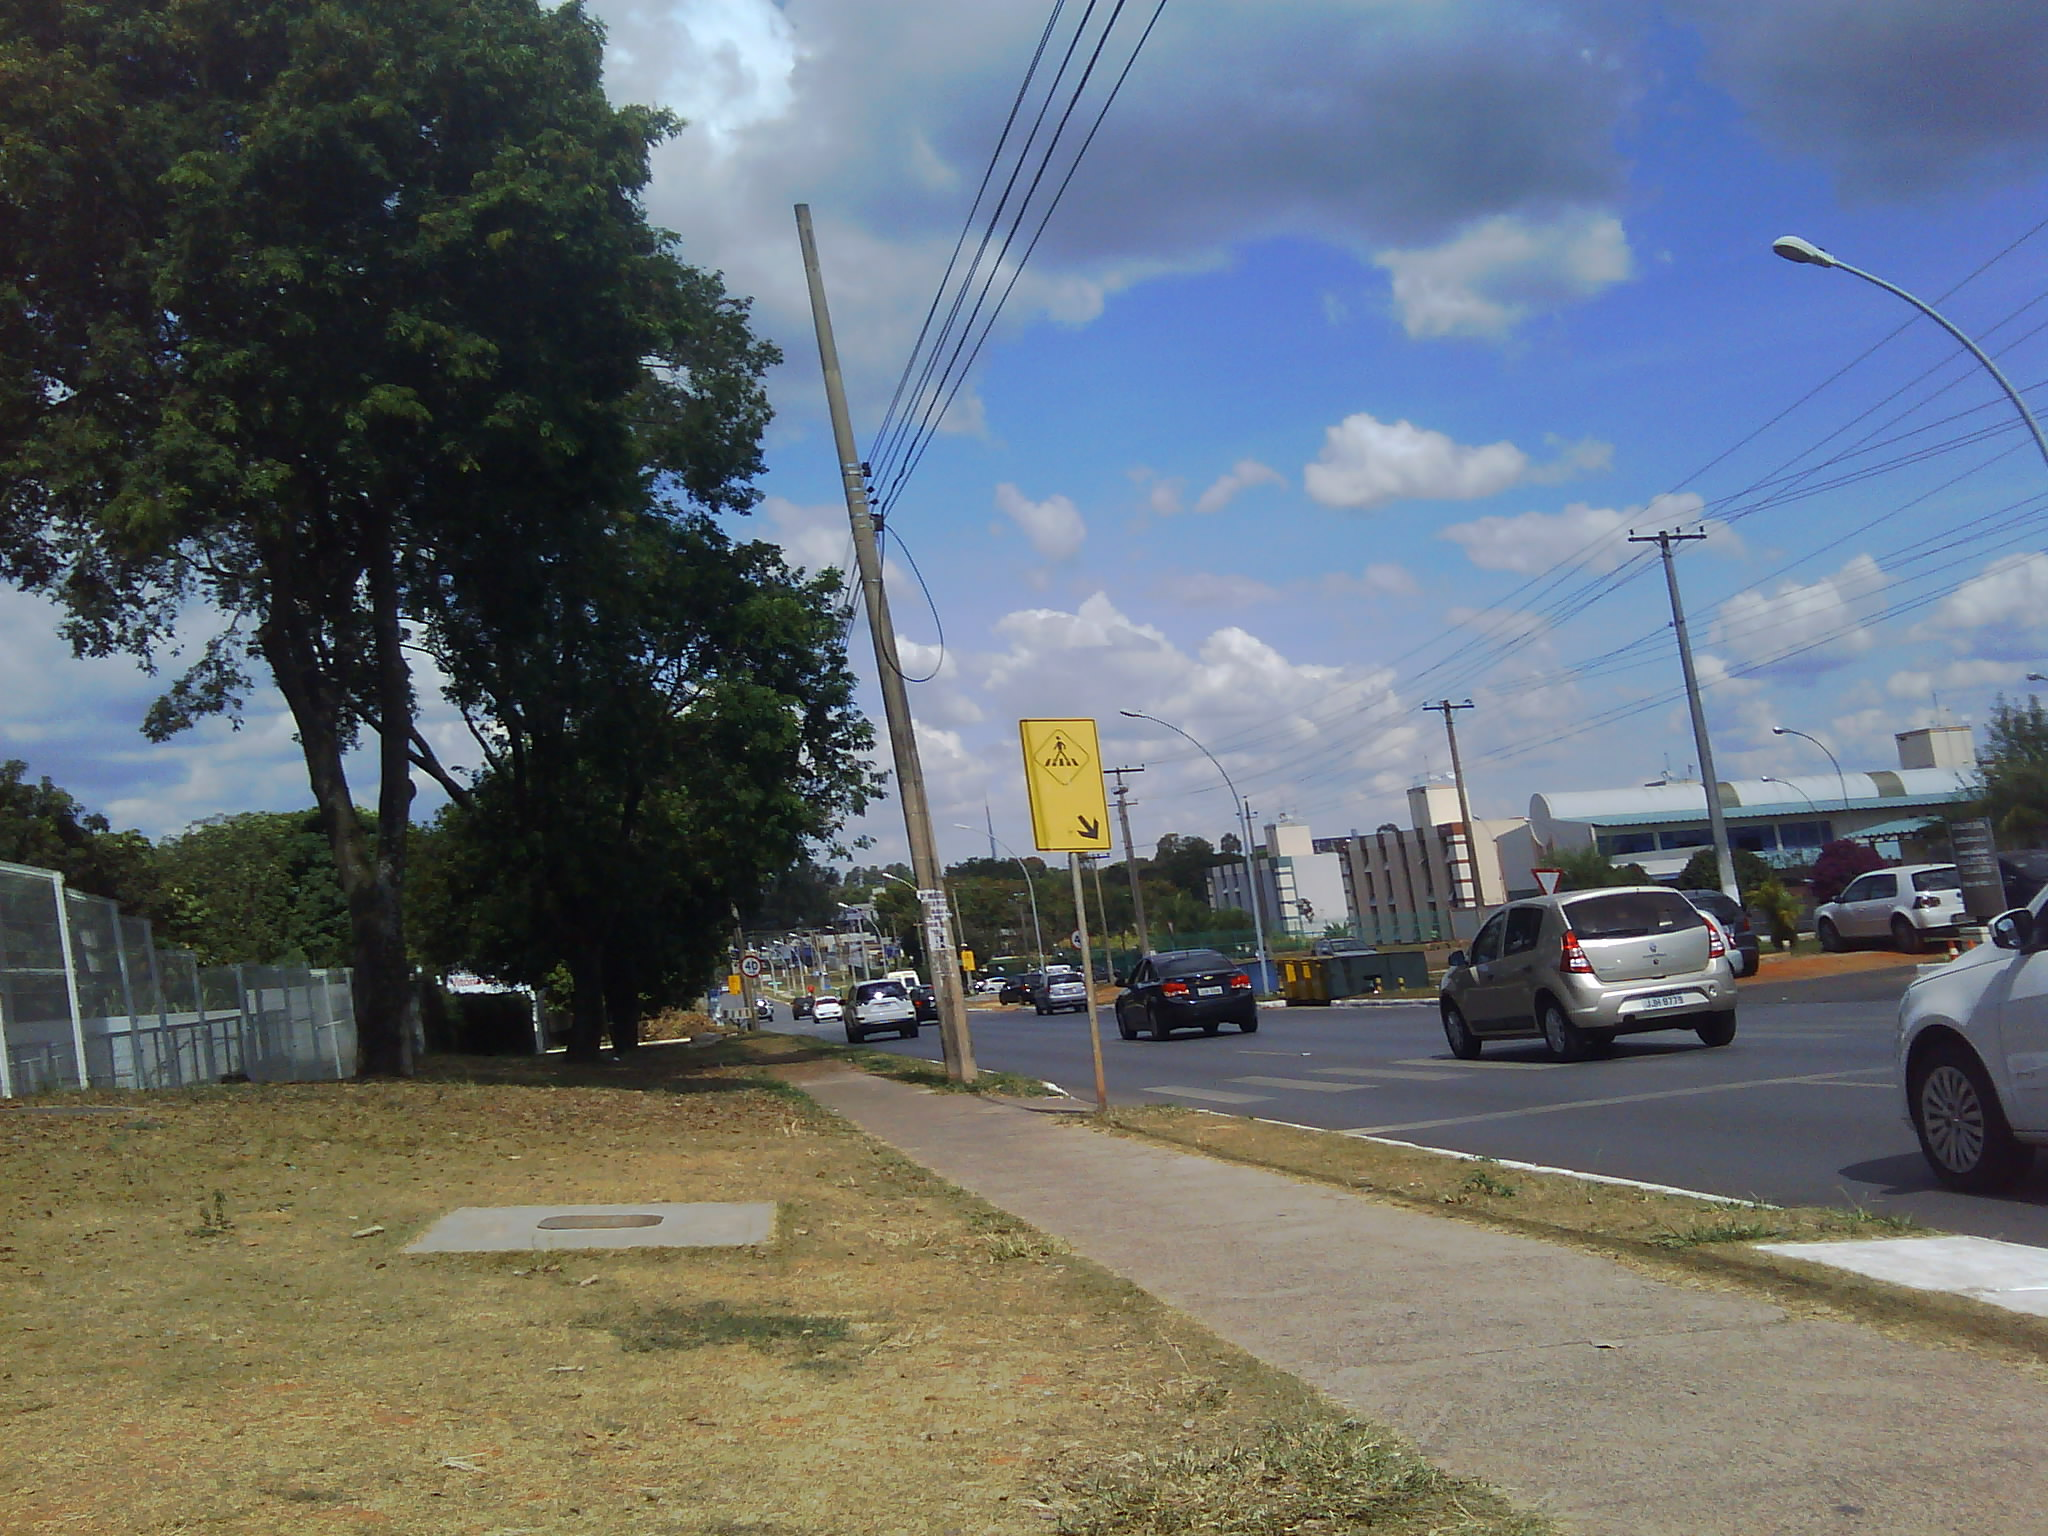
\includegraphics[width=.5\textwidth]{imagens/2016-05-15T12-57-10.jpeg}
        \caption{fluxo de veículos na rodovia W5}
        \label{figura05}
\end{figure}
\paragraph{}A  grande  maioria  dos  seus  discente  tem  suas  moradias  distante  da  escola,  isto  se dar  devido  ao  processo  de  seleção  do  Governo  do  Distrito  Federal  (GDF).  Eles  vem  da diversas  cidades  satélites  e  do  entorno,  tais  como:  Vicente  Pires,  Paranoá,  Itapuã,  Jardim Botânico,  Cidade   Ocidental.   Isto  faz  com  que  muitos  alunos  passem   horas,  em  média   2hs, em  transito  (casa-escola-casa).  Isto  se  dar  pelo  processo  de  seleção  do  governo,  que prioriza  a  proximidade  da  habitação  ou  trabalho  dos  pais.  Segundo  Júlio,  vigilante  da escola,  os  país  colocam  seus  filhos próximo aos trabalhos, para com  isso ficar de olhos nos mesmos, figura \ref{figura06}.  Devido  os  alunos  morarem  em  diferentes  localidades,  eles  não  se sentem  parte  integrante  da  comunidade  escolar  local,  transformando  a  escola  como  um local de passagem.
\begin{figure}[!htpb]
        \centering
        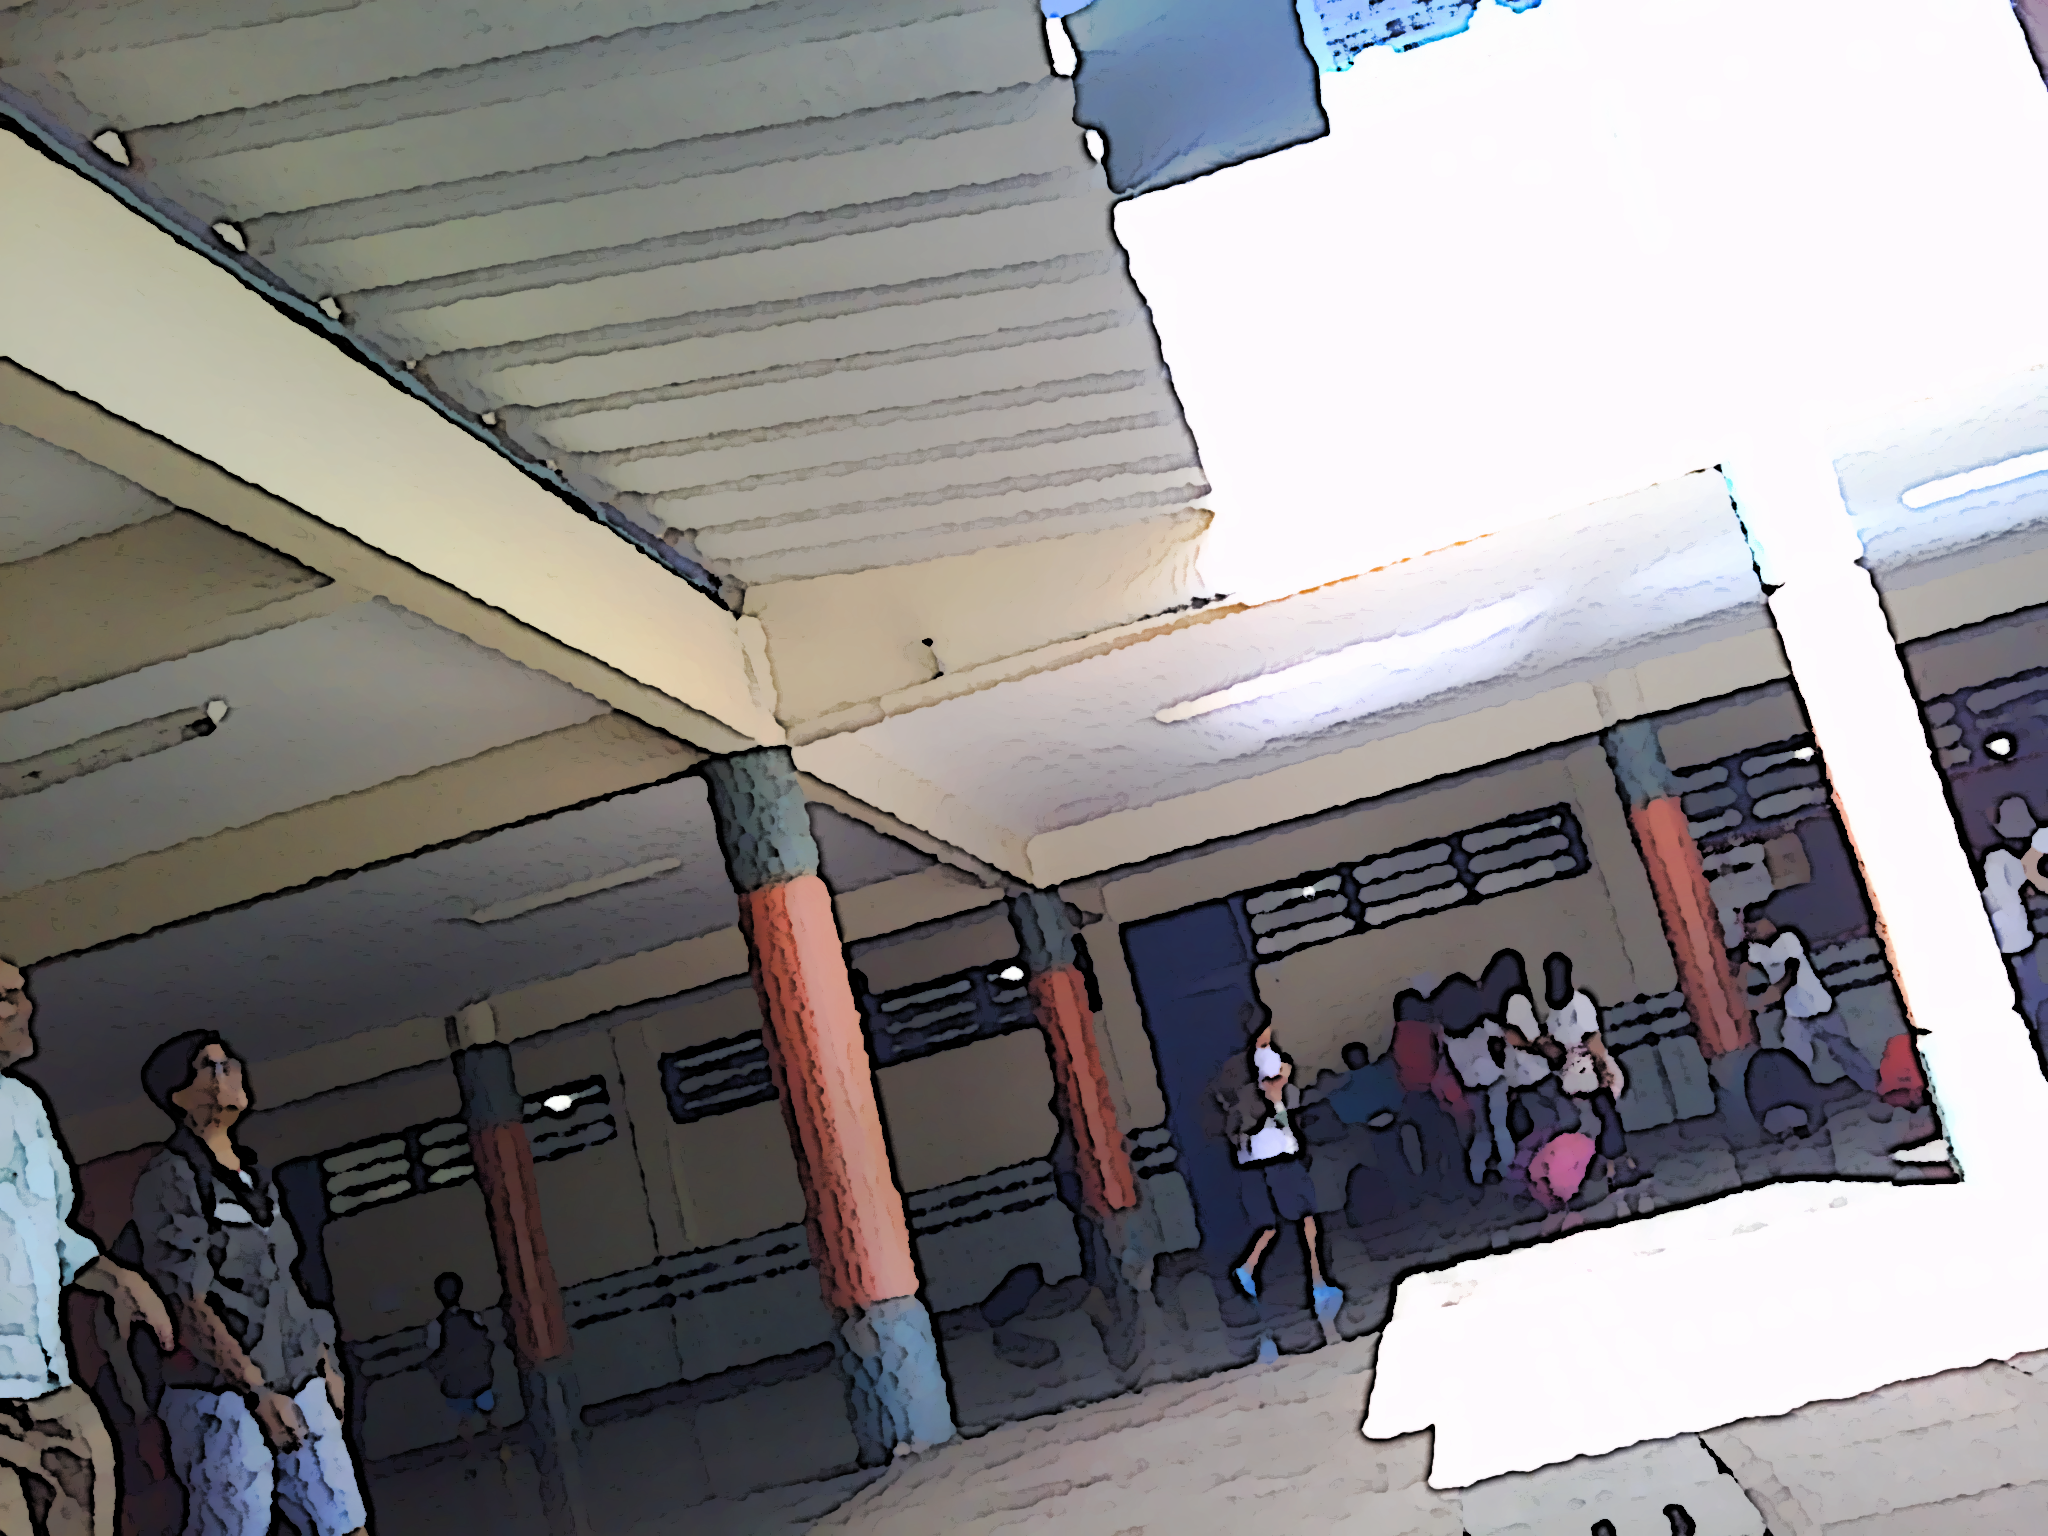
\includegraphics[width=.7\textwidth]{imagens/paiealunoEntrada01.png}
        \caption{Pai com aluno na entrada da escola}
        \label{figura06}
\end{figure}
\paragraph{}O  corpo  de  funcionários  da  escola  (professores,  secretária),  também  tem  sua residências  nas  cidades  satélites,  tais  como:  Sobradinho,  Guará  e  Jardim  Mangueiral,  com deslocamento de carro.  Já  os  vigilantes  e  pessoal  do  serviço  gerais,  possuem  suas moradias,  basicamente,   nas  mesmas   localidades  dos  alunos.  O  primeiro  grupo  tem  sua rotina  escolar  muito  dinâmica,  com  chegada  e   saída  somente  para  as  aulas.   Muitos  deles sequer  conhece  seus  companheiro  de  outros  turno. Já o segundo grupo passa pelo mesma questão  dos  alunos  que  passam  muito  tempo  em  deslocamento.  Porém  todos  eles  se sentem parte integrantes do ambiente escolar.